



%--------------------------------------


\newpage

\section[Network Growth Models][Modèles de Croissance de Réseau]{Network Growth Models : Explicative power for various approaches}{Modèles de Croissance de Réseau}

\label{sec:networkgrowth}


%--------------------------------------

Nous proposons dans un premier temps de détailler la composante réseau pour l'échelle mesoscopique.


%--------------------------------------

%%%%%%%%%%%%%%%%%%%%
\subsection{Benchmarking Network growth heuristics}{Comparer les heuristiques de croissance de réseau}


\bpar{
Considering Network Growth in itself, many heuristics are available to generate a network under some constraints. As already developed, from economic network growth approach to local optimization heuristics, geographical mechanisms or biological network growth, each has its advantages and particularities.
}{
Pour la croissance du réseau en tant que tel, de nombreuses heuristiques existent pour générer un réseaux sous certaines contraintes. Comme déjà développé précédemment, des modèles économiques de croissance de réseau au heuristiques d'optimisation locale, aux mécanismes géographiques ou à la croissance de réseau biologique, chacun a ses avantages et particularités propres. Nous avons déjà testé en~\ref{sec:correlatedsyntheticdata} une heuristique basée sur la rupture de potentiel d'interaction. Pour pouvoir comparer ``toutes choses égales par ailleurs'' les différentes heuristiques de génération de réseau, il est nécessaire des les explorer à densité fixée, même si le sens thématique des résultats ne peut avoir de valeur sur le temps long.
}


L'importance d'heuristiques pouvant capturer une structure topologique permettant un certain compromis entre performance, congestion et coût, est montrée par des analyses empiriques comme \cite{2012arXiv1202.1747W} pour les réseaux de métro, qui montre que les motifs d'évolution des corrélation entre degrés témoignent d'une évolution des réseaux vers une telle topologie.




%%%%%%%%%%%%%%%%%%%%%%%
\subsubsection{Euclidian heuristic}{Heuristique euclidienne}

Nous appliquons la méthode développée en~\ref{sec:correlatedsyntheticdata}.



%%%%%%%%%%%%%%%%%%%%%%%
\subsubsection{Biological heuristic}{Heuristique biologique}

\cite{raimbault2015labex} explore des applications des modèles de croissance de réseau biologique, notamment leur capacité à produire de manière émergente des solutions optimales au sens de Pareto pour des indicateur contradictoires, comme le coût et la robustesse. Un aperçu des potentialités est donné en Appendice~\ref{app:sec:biological}. Etant donné un réseau initial dont les liens ont des capacités uniformes, l'itération d'équilibres de pression successifs suivis d'une évolution des capacités, permet une convergence vers une distribution hiérarchique stable des capacités. Notre rationnelle est d'utiliser ce mécanisme pour à un instant donné déterminer un certain nombre de liens réalisés, en fonction d'une nouvelle configuration. Les avantages de l'heuristique que nous allons détailler sont notamment que (i) elle peut être utilisée de manière itérative pour traduire une évolution topologique séquentielle du réseau, en comparaison à la plupart des modèles d'investissement qui font évoluer uniquement les capacités dans le temps.






%%%%%%%%%%%%%%%%%%%%%%%
\subsection{Results}{Résultats}


\subsubsection{Experience plan}{Plan d'expérience}


% à longueur de réseau fixée ? difficile car pas controlé directement.
% test sur quelques config de densité typique ?



\subsubsection{Feasible space}{Topologies obtenues}




%%%%%%%%%%%%%%%%%
\begin{figure}
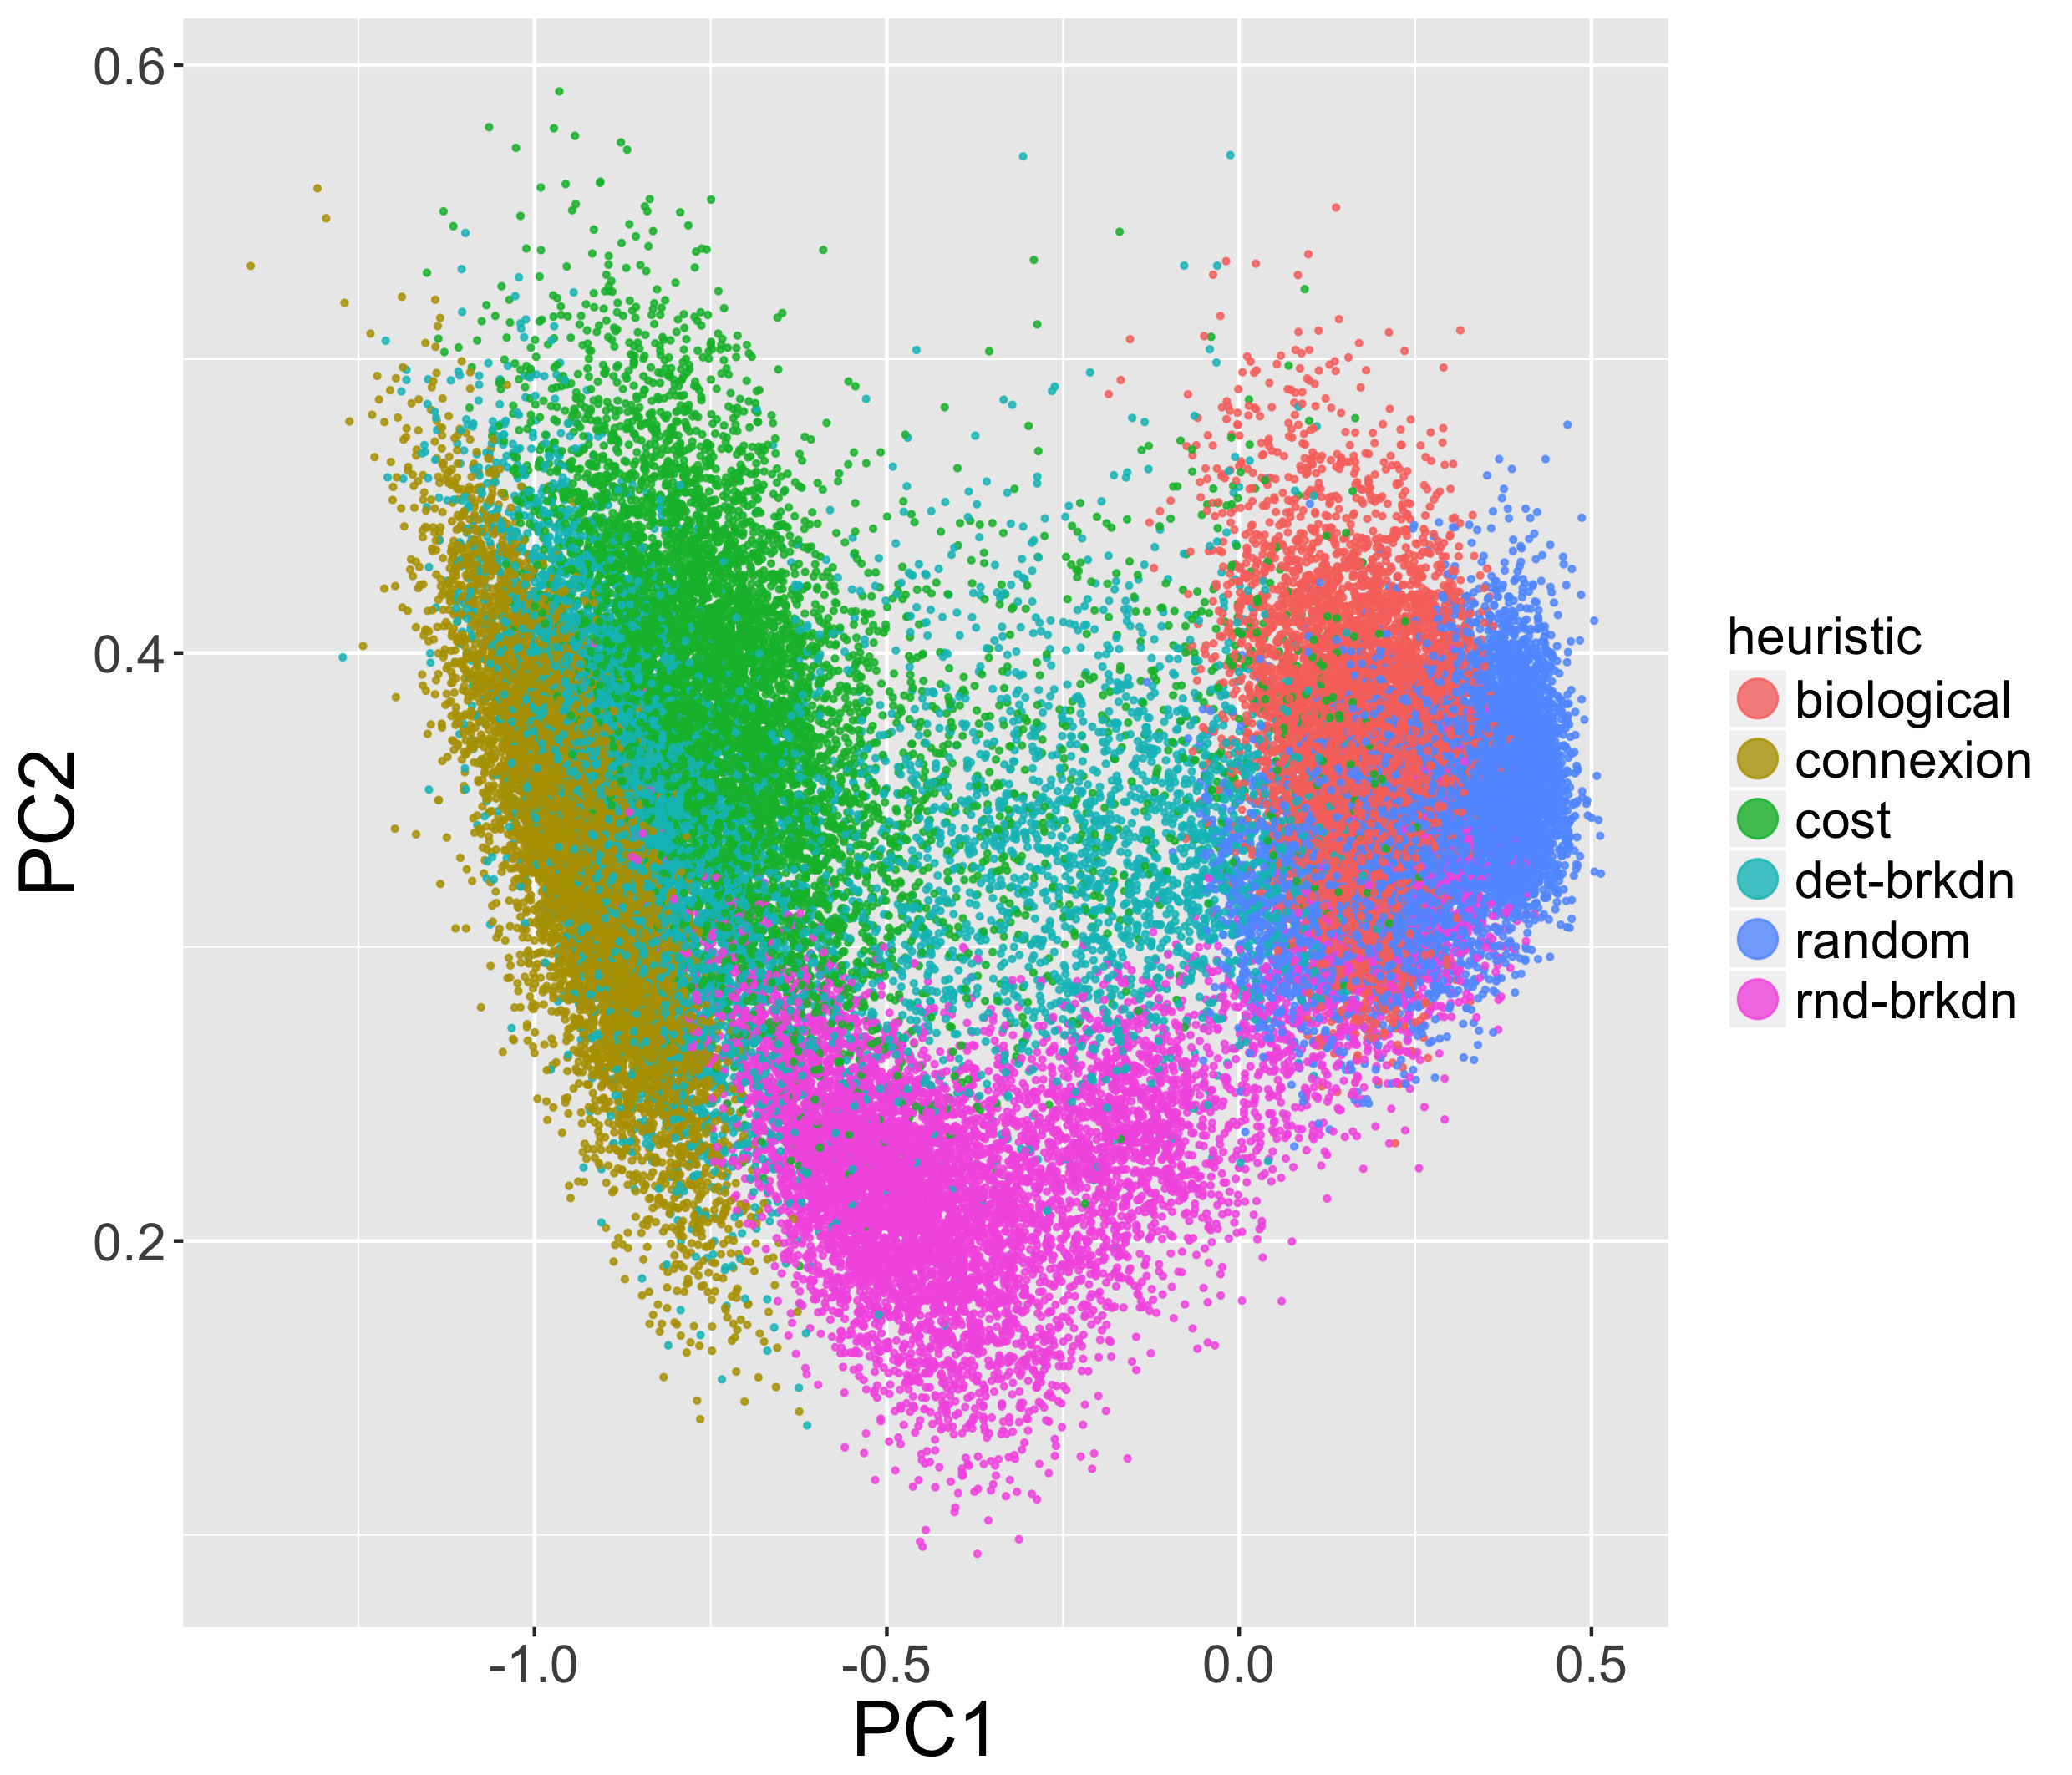
\includegraphics[width=\linewidth]{Figures/NetworkGrowth/feasible_space_pca}
\caption[][Espace topologique faisable]{}{\textbf{Espace topologique faisable pour les différentes heuristiques de génération.} La même figure conditionnée à la classe morphologique de densité est donnée en Appendice~\ref{app:sec:networkgrowth}.\label{fig:networkgrowth:feasiblespace}}
\end{figure}
%%%%%%%%%%%%%%%%%

% PCA synth
%
%                                PC1        PC2        PC3        PC4         PC5
%meanBwCentrality        -0.51420330 -0.4500671  0.5415210 -0.4602950  0.16708710
%meanPathLength          -0.45662839  0.1782617 -0.2556133  0.3151101  0.77141477
%meanRelativeSpeed        0.57854267  0.3344679  0.3147784 -0.4083421  0.53627500
%nwDiameter              -0.43570261  0.8011179  0.1305644 -0.2508956 -0.29728372
%meanClosenessCentrality  0.05036956  0.1095611  0.7247651  0.6776003 -0.03213514
%Importance of components:
%                          PC1     PC2     PC3     PC4     PC5
%Standard deviation     0.4981 0.06762 0.04611 0.03423 0.02982
%Proportion of Variance 0.9659 0.01780 0.00828 0.00456 0.00346
%Cumulative Proportion  0.9659 0.98370 0.99198 0.99654 1.00000



\subsubsection{Real network comparison}{Comparaison aux réseaux réels}







%%%%%%%%%%%%%%%%%
\begin{figure}
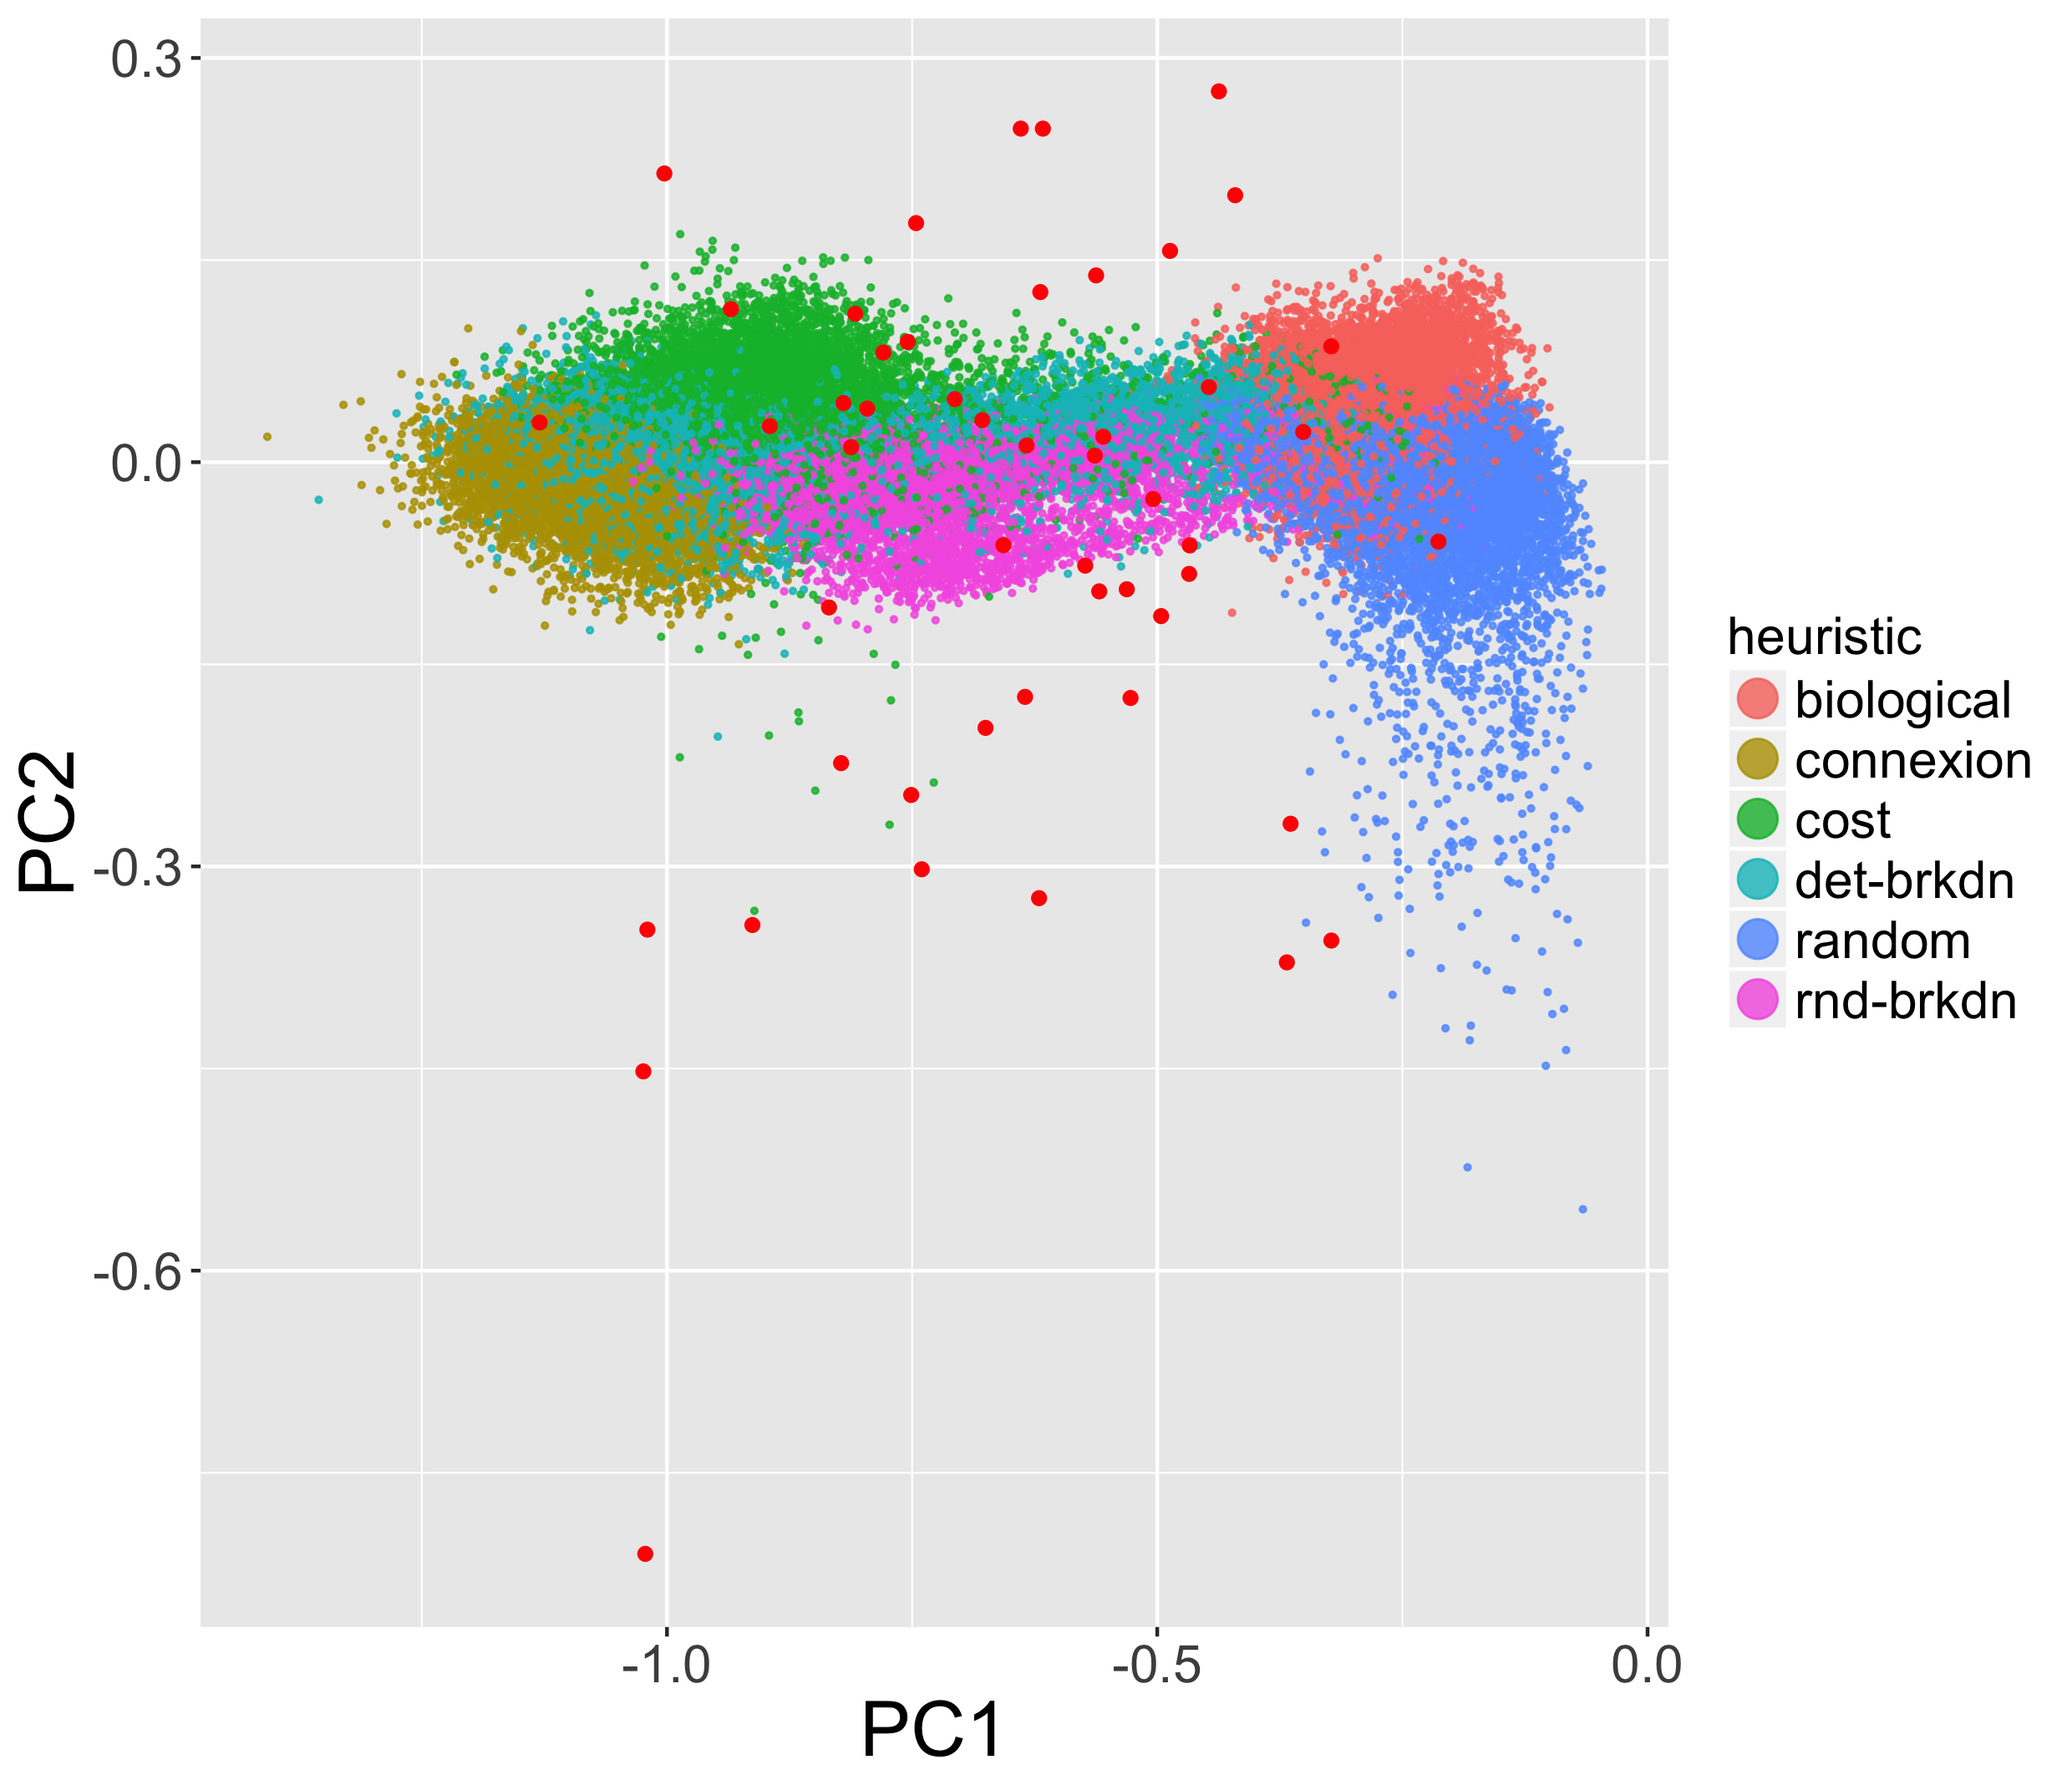
\includegraphics[width=0.45\linewidth]{Figures/NetworkGrowth/feasible_space_withreal_pca}
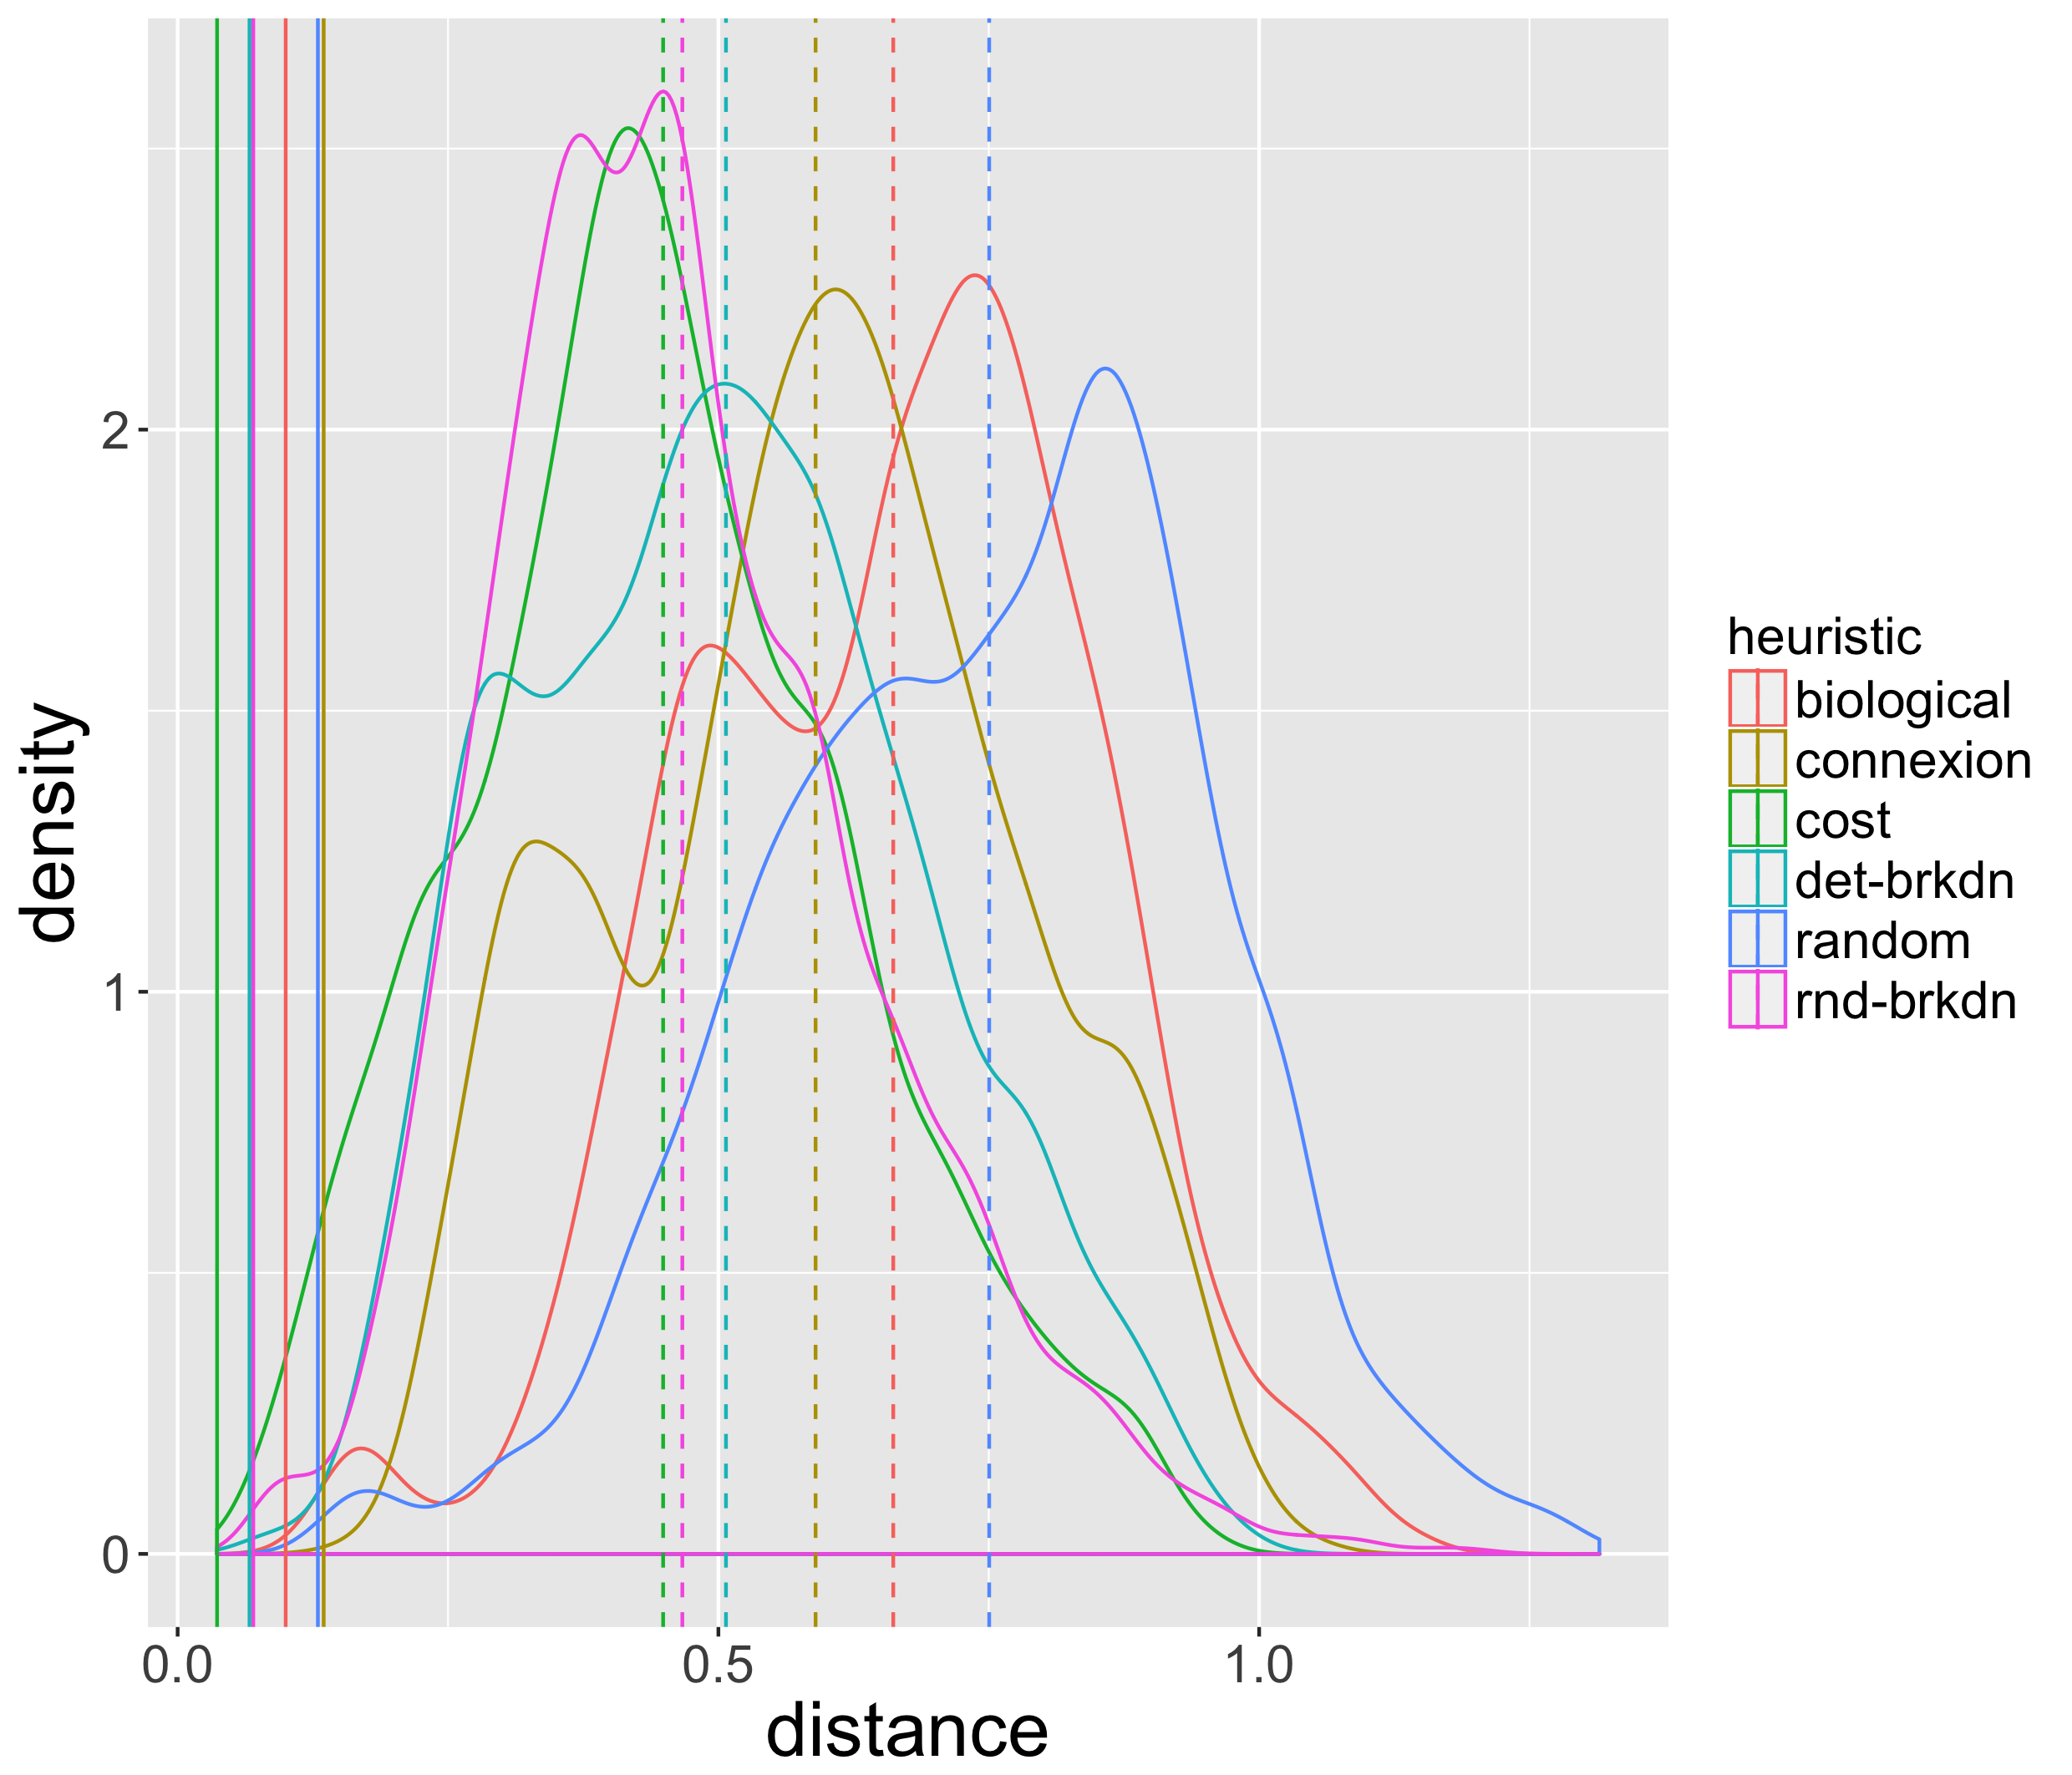
\includegraphics[width=0.45\linewidth]{Figures/NetworkGrowth/distance_real}\\
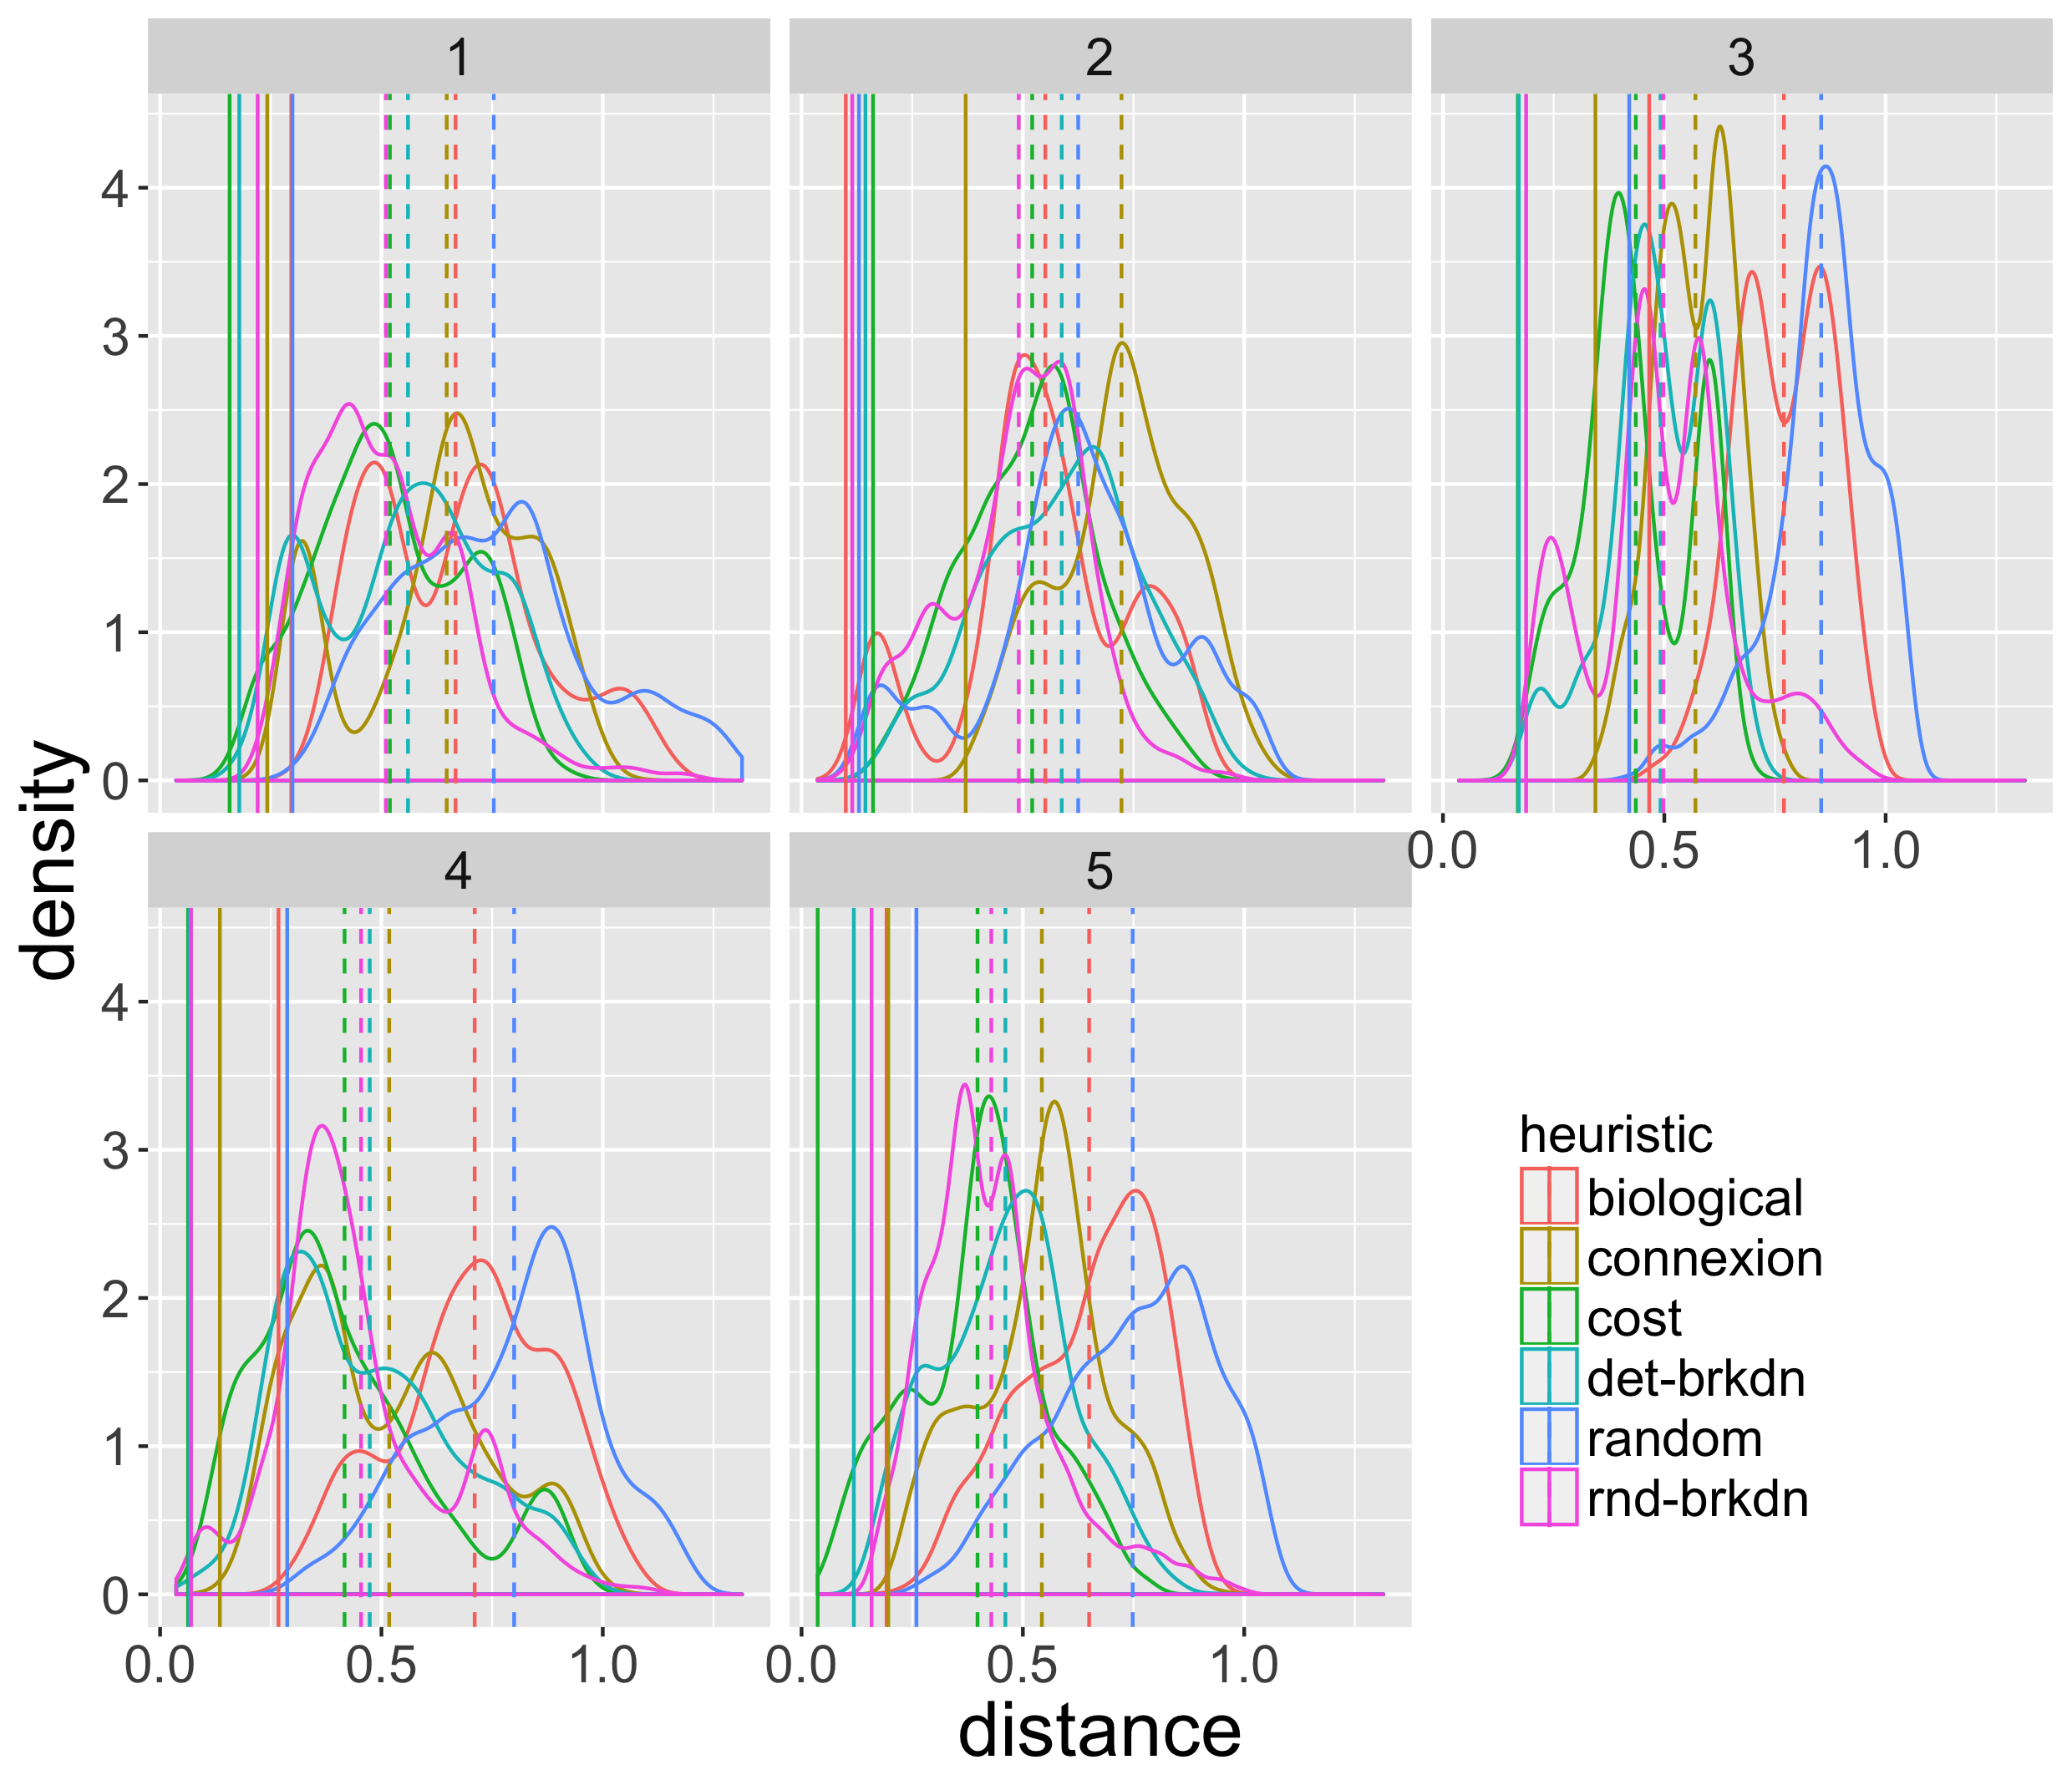
\includegraphics[width=0.45\linewidth]{Figures/NetworkGrowth/distance_real_bymorph}
\caption[][Comparaison aux réseaux réels]{}{\textbf{Comparaison aux réseaux réels.} \label{fig:networkgrowth:realdistance}}
\end{figure}
%%%%%%%%%%%%%%%%%



% PCA real

%Rotation:
%                        PC1        PC2          PC3         PC4         PC5
%meanBetweenness  0.32071179  0.9123552 -0.101287507  0.09905262 -0.21137945
%meanPathLength   0.67349835 -0.3016661 -0.670421641  0.04531017  0.06228457
%meanCloseness   -0.01926100  0.2063540 -0.009888761  0.19655887  0.95828695
%networkPerf     -0.05108717 -0.1222155  0.053354929  0.97433440 -0.17400925
%diameter         0.66374922 -0.1381554  0.733028737 -0.01314015  0.05335036
%Importance of components:
%                          PC1     PC2     PC3     PC4     PC5
%Standard deviation     0.1084 0.08207 0.05094 0.03375 0.02602
%Proportion of Variance 0.5132 0.29415 0.11332 0.04976 0.02957
%Cumulative Proportion  0.5132 0.80736 0.92067 0.97043 1.00000
%


% Distances

%nres%>%group_by(heuristic)%>%summarise(distance=min(distance))
%1 biological 0.09990225
%2  connexion 0.13504050
%3       cost 0.03647362
%4  det-brkdn 0.06644744
%5     random 0.12968739
%6  rnd-brkdn 0.06994303
%
%nres%>%group_by(heuristic)%>%summarise(distance=mean(distance))
%
%1 biological 0.6616921
%2  connexion 0.5898689
%3       cost 0.4489075
%4  det-brkdn 0.5070177
%5     random 0.7504109
%6  rnd-brkdn 0.4666547
%
%nres%>%group_by(heuristic)%>%summarise(distance=median(distance))
%
%1 biological 0.6780299
%2  connexion 0.5973273
%3       cost 0.4359749
%4  det-brkdn 0.5024551
%5     random 0.7680822
%6  rnd-brkdn 0.4462033


%%%%%%%%%%%%%%%%%%%%%%%
\subsection{Discussion}{Discussion}



Limitation du slime-mould \cite{adamatzky2010road}










